\subsection{Stabilità}

Mostriamo l'instabilità del nostro sistema di rivelatori nei 2 apparati sopra descritti monitorando la posizione dei fotopicchi del sodio in funzione del tempo.
La prima misura è stata fatta con il circuito A il 3 maggio e dura \SI{16}{ore}, la seconda  è stata eseguita con il circuito B il 15 maggio e dura \SI{63}{ore}.
Nella prima misura sono presenti tutti i canali, nella seconda è presente solo il canale 1 per evitare il cross-talk riscontrato nella precedente.
Abbiamo usato l'energia nominale dei 2 picchi per ricavare una retta di calibrazione\footnotemark
\footnotetext{Qui diamo per nota la massa dell'elettrone anche se misurarla è tra gli scopi dell'esperienza.}
di pendenza $m$ e intercetta $q$ e abbiamo osservato l'evoluzione temporale di questi parametri.
%Usiamo l'espressione tra virgolette perché lo scopo dell'esperienza è fingere di non conoscere la massa dell'elettrone per poi misurarla.

% misura 1
\begin{figure}[h]
\centering
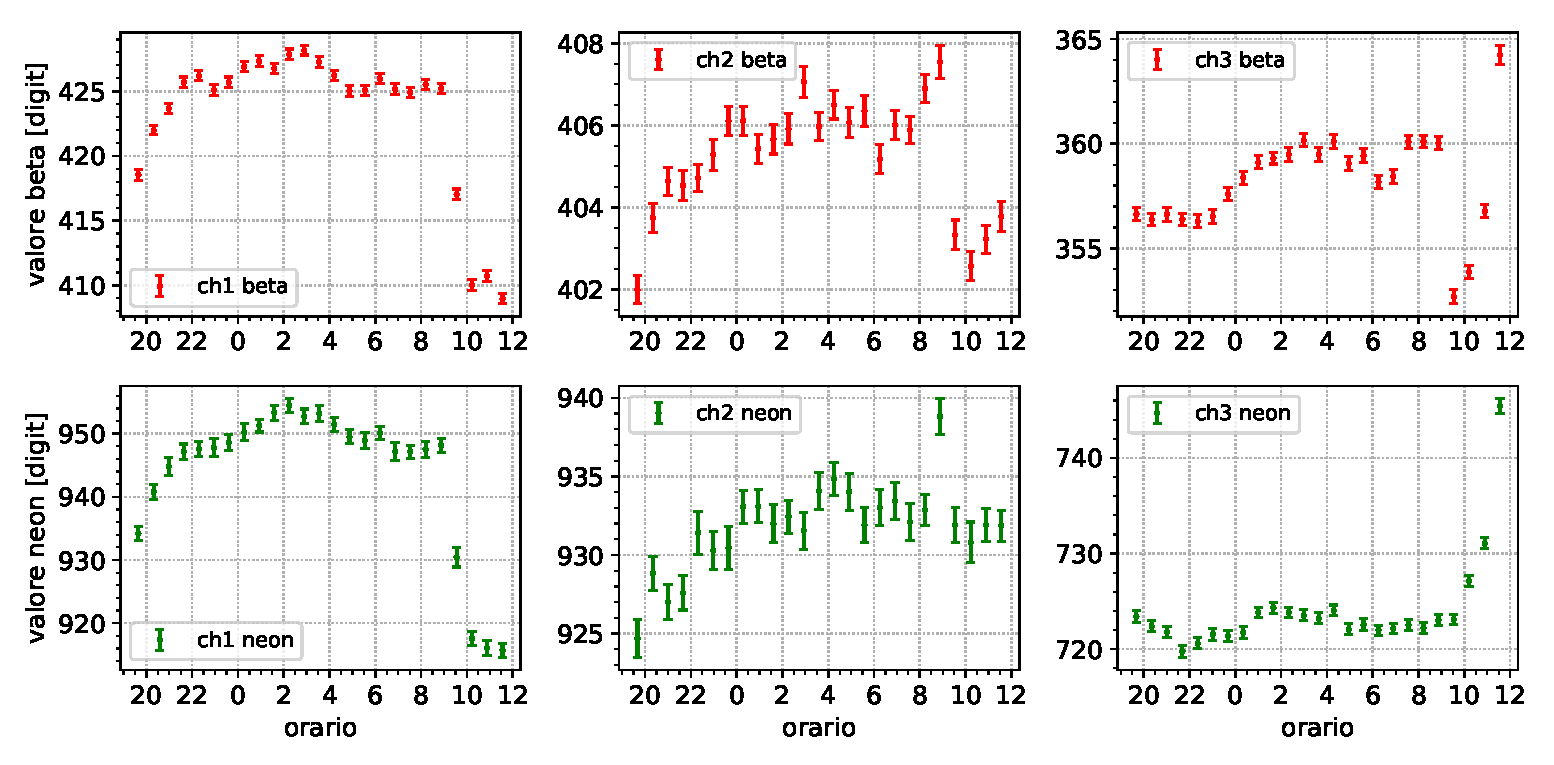
\includegraphics[width=\textwidth]{immagini/0503_picchi}
\caption{Misura di stabilità iniziata il 3 maggio alle 19. I grafici rappresentano la posizione dei picchi in funzione del tempo; ``beta'' indica il picco di annichilazione e ``neon'' indica il fotone emesso dal decadimento del neon.}
\label{picchi1}
\end{figure}

\begin{figure}[h]
\centering
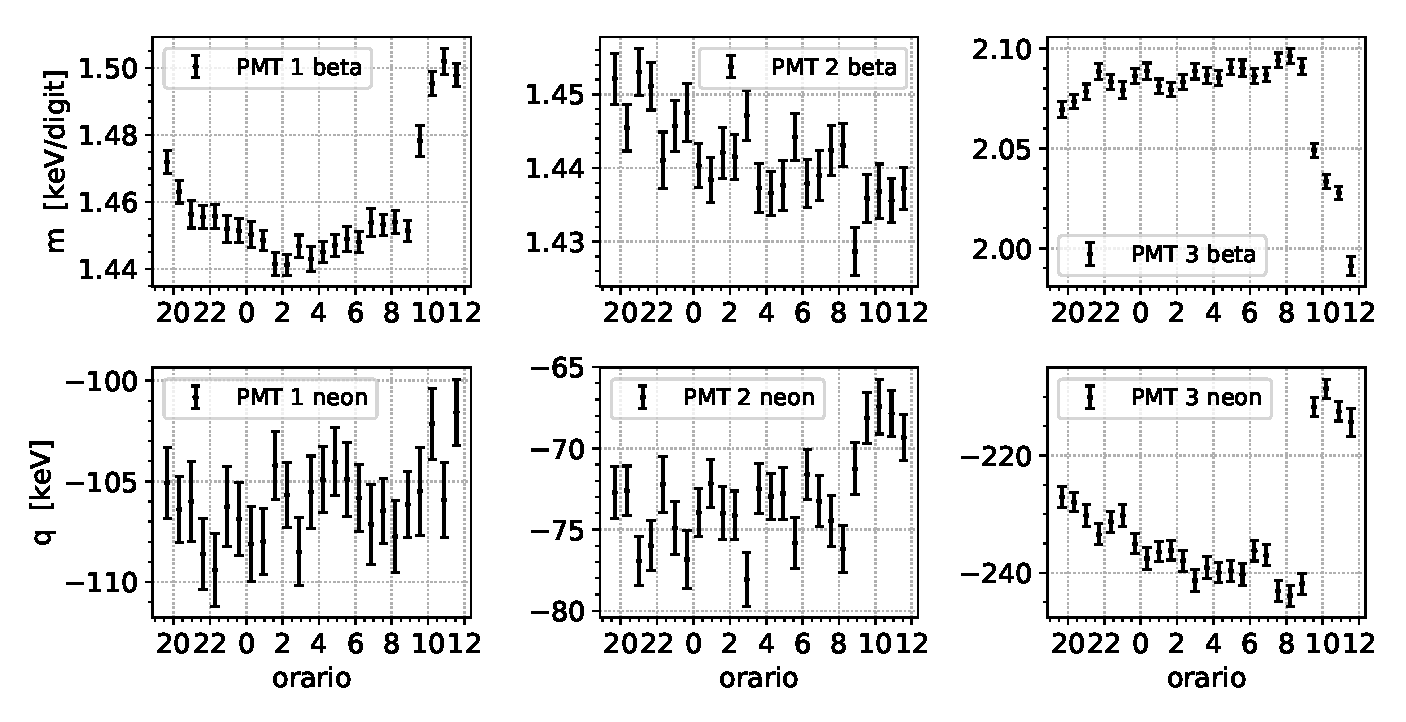
\includegraphics[width=\textwidth]{immagini/0503_rette}
\caption{Misura di stabilità iniziata il 3 maggio alle 19. I grafici rappresentano il valore della pendenza e dell'intercetta della ``retta di calibrazione'' in funzione del tempo.}
\label{rette1}
\end{figure}

% misura 2
\begin{figure}[h]
\centering
\subfloat
{
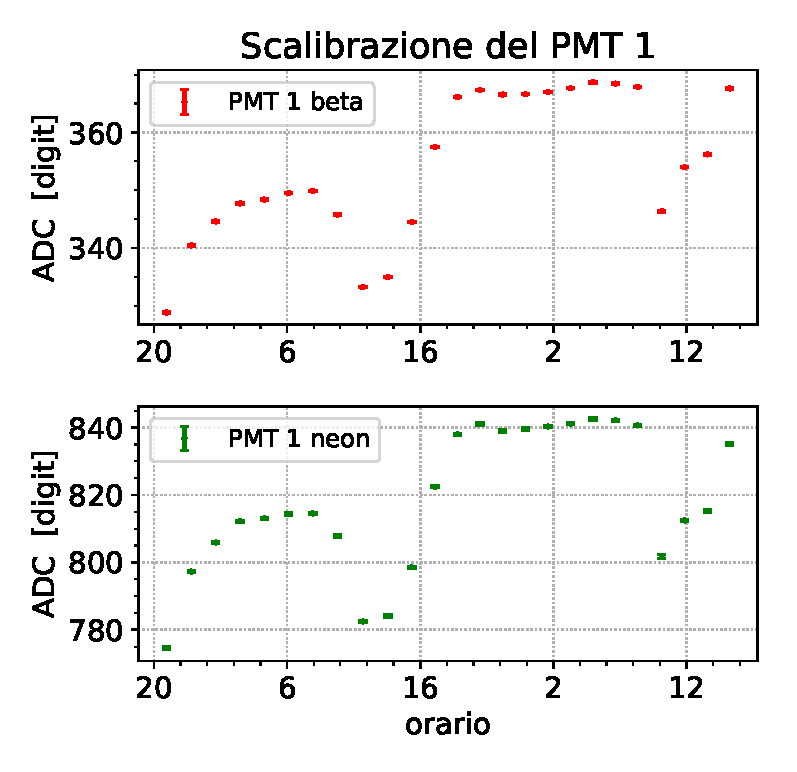
\includegraphics[width=0.49\textwidth]{immagini/0515_picchi}
}
\subfloat
{
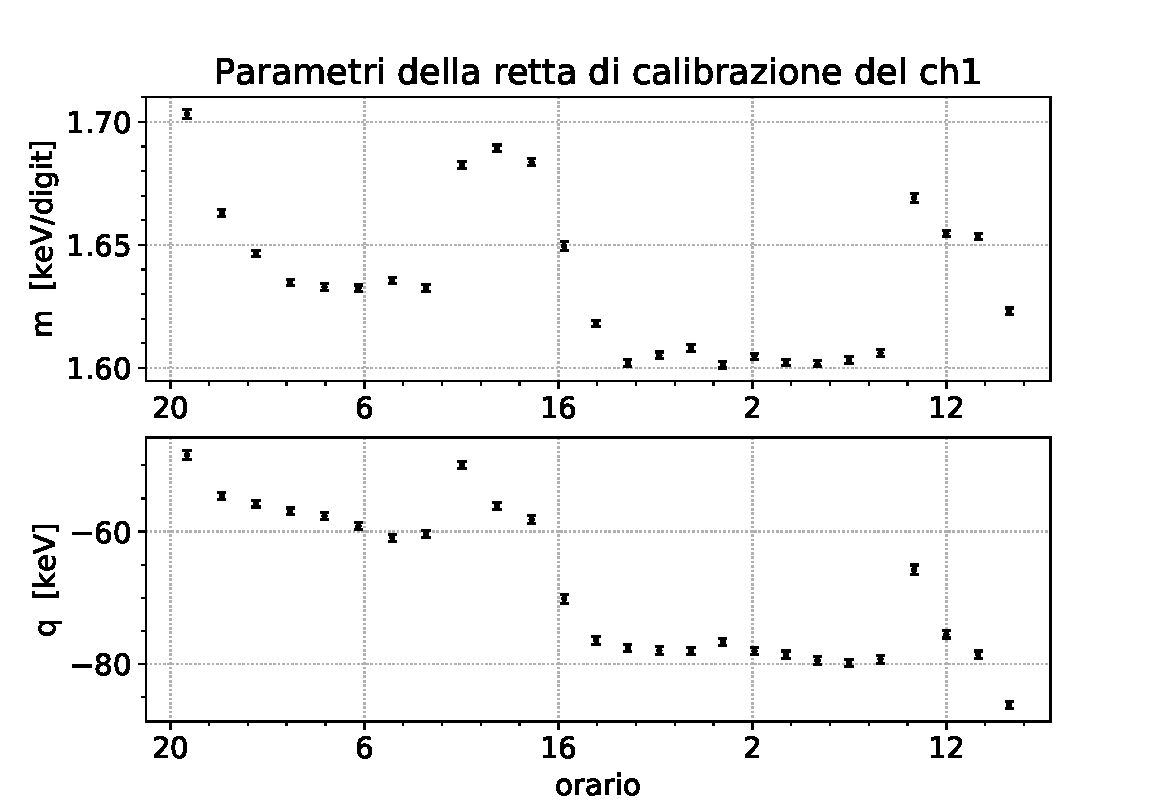
\includegraphics[width=0.49\textwidth]{immagini/0515_rette}
}
\caption{Misura di stabilità iniziata il 15 maggio alle 19.
\emph{A sinistra}:  grafici che rappresentano la posizione dei picchi in funzione del tempo; ``beta'' indica il picco di annichilazione e ``neon'' indica il fotone emesso dal decadimento del neon.
\emph{A destra}: grafici che rappresentano il valore della pendenza e dell'intercetta della retta di calibrazione in funzione del tempo.}
\label{picchi2}
\end{figure}

% discussione dei dati
Guardando i dati della prima misura (\autoref{picchi1} e \autoref{rette1}) vediamo che i vari rivelatori si scalibrano in modo diverso. L'andamento dei punti indica la notte come momento di massima stabilità e l'apertura del laboratorio come momento di massima instabilità.
Dai dati della seconda misura (\autoref{picchi2} sinistra e \autoref{picchi2} destra) si nota uno spostamento coerente dei fotopicchi del sodio che si stabilizza durante la notte. Anche qui si nota una scalibrazione significativa durante gli orari di apertura del laboratorio.
Le stesse considerazioni valgono anche per i parametri della retta di calibrazione.